
\begin{transitionframe}
\textbf{Part F:}

Conclusions
\end{transitionframe}



\begin{frame}{Summary of Results about the Ontological Proof}
\begin{itemize}[<+->]
\item K sufficient for T1, C1 and T2 
\item S5 not needed for T3
\item KB sufficient for T3 
\item A simpler new proof of C1
\item G\"odel's original axioms (without conjunct $\phi(x)$ in D2) are inconsistent
\item Scott's axioms are consistent
\item For T1, only half of A1 (A1a) is needed 
\item For T2, the other half (A1b) is needed
\end{itemize}
\end{frame}


\begin{frame}{Summary of Results for Logic} \small
\begin{itemize}[<+->]
\item Infra-structure for reasoning with modal logic using existing proof assistants and higher-order automated theorem provers
\item A new natural deduction calculus for higher-order modal logic
\item Difficult benchmarks for higher-order automated theorem provers
\end{itemize}
\end{frame}

\begin{frame}{Conclusion} \large
What have we achieved \\[.5em]
\begin{itemize}
\item Verification of G\"odel's ontological argument with HOL provers
  \begin{itemize}
  \item exact parameters known: constant domain quantification, Henkin Semantics
  \item parameters can be varied and experiments can repeated
  \end{itemize}
\item Gained some novel results and insights
\item Major  step towards \alert{Computer-assisted Theoretical Philosophy}
 \begin{itemize}
  \item see also Ed Zalta's \emph{Computational Metaphysics} project at Stanford University
  \item remember Leibniz' dictum --- \emph{Calculemus!}
  \end{itemize}
\item Highly fascinating bridge between CS, Philosophy and Theology
\item Major public interest 
\end{itemize}
\vfill
Future Work
\begin{itemize}
\item 
\end{itemize}
\end{frame}

\begin{frame}[plain]
\colorbox{black}{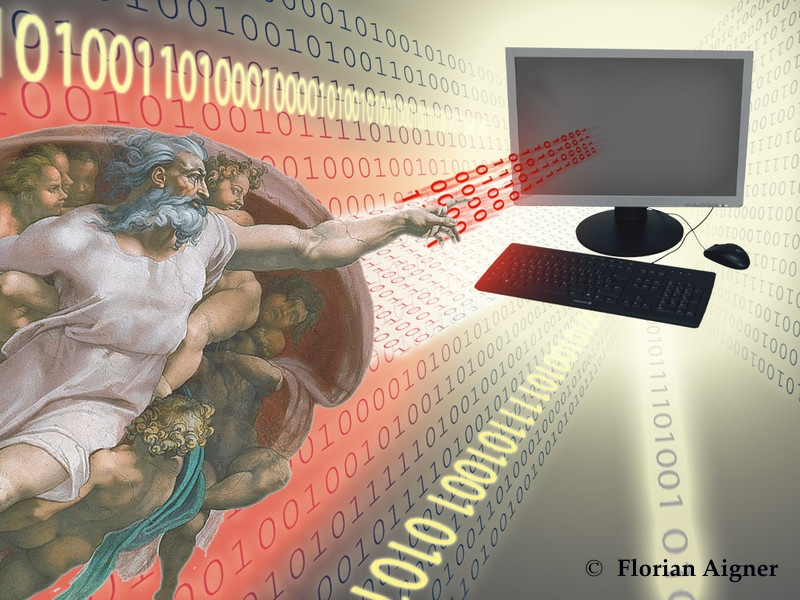
\includegraphics[width=\textwidth]{TUWien-GodComputerC}}
\end{frame}
